\documentclass[9pt]{extarticle}

% Encoding and languages
\usepackage[T1]{fontenc}
\usepackage[utf8]{inputenc}
\usepackage[french]{babel}
% Mathematics
\usepackage{amsmath,amssymb}
% Hyperlinks and PDF
\usepackage{lastpage}
\usepackage{hyperref}
\usepackage{bookmark}
% Lists
\usepackage{enumitem}
% Page layout
\usepackage[a4paper, margin=2.5cm]{geometry}
% Line spacing and formatting
\usepackage{setspace}
\onehalfspacing             % 1.5 line spacing for a scientific article
\setlength{\parindent}{0pt} % no indentation
\setlength{\parskip}{6pt}   % vertical spacing between paragraphs
% Figures and TikZ
\usepackage{graphicx}
\usepackage{tikz}
\usepackage{float}
\usetikzlibrary{decorations.pathreplacing,trees,calc}
\usetikzlibrary{arrows.meta, positioning}
\usetikzlibrary{matrix, positioning, arrows.meta}
\usepackage[numbers]{natbib}

% Colors and boxes
\usepackage[many]{tcolorbox}
\tcbset{
  mydefstyle/.style={
    colback=white,
    colframe=black,
    fonttitle=\bfseries,
    boxrule=0.8pt,
    arc=4pt,
    left=3mm, right=3mm, top=5mm, bottom=5mm,
    breakable
  }
}
\newtcolorbox{defbox}[2][]{mydefstyle,title=#2,#1}

% Section titles
\usepackage{titlesec}
\titlespacing*{\section}{0pt}{1.5ex plus 1ex minus .2ex}{1ex plus .2ex}
\titlespacing*{\subsection}{0pt}{1ex plus .5ex minus .2ex}{0.5ex plus .2ex}
\titlespacing*{\subsubsection}{0pt}{0.8ex plus .3ex minus .1ex}{0.3ex plus .1ex}

% Headers and footers
\usepackage{fancyhdr}
\setlength{\headheight}{14pt}
\pagestyle{fancy}
\fancyhf{}
\fancyhead[L]{Constrained Pseudorandom Functions, Revisited}
\fancyhead[R]{Sorbonne Université}
\fancyfoot[C]{\thepage\ /\ \pageref{LastPage}}

% TikZ states and arrows
\tikzset{ 
  state/.style={
    draw,
    rectangle,
    rounded corners,
    minimum height=8mm,
    minimum width=14mm,
    align=center,
    font=\small,
  },
  hashstate/.style={
    state,
    fill=red!20
  },
  arrow/.style={
    ->,
    thick
  }
}

%========================================================================================

\title{Constrained Pseudorandom Functions, Revisited}
\author{
\textbf{Julian Mouthon, Mario Razafinony}\\
\small Master 1 in Cryptology, High-Performance Computing and Algorithms\\
\small Sorbonne Université\\
}
\date{\today}

\begin{document}

\begin{figure}
  \centering
  
\includegraphics[width=0.4\textwidth]{./images/sorbonne.png}
\end{figure}

\maketitle

\section*{Introduction}
Pseudorandom functions (PRFs) are fundamental primitives in modern cryptography.
They are used in many protocols, notably for symmetric encryption, authentication, and key derivation.

In some contexts, it is necessary to delegate only part of the evaluation capabilities of a PRF without revealing the full secret key. This need arises in particular in the context of Searchable Symmetric Encryption and outsourced storage on untrusted servers, where it is necessary to precisely control an adversary’s evaluation capabilities~\cite{BMO17}.

Constrained pseudorandom functions (CPRFs) address this problem by allowing the restriction of the function’s evaluation to a subset of inputs defined by a constraint~\cite{BMO17}.

This project focuses on the CPRF construction proposed by
Bost, Minaud, and Ohrimenko in 2017~\cite{BMO17}, based on iteration of a trapdoor permutation.

First, we present the fundamental notions related to pseudorandom functions and CPRFs, as well as the construction introduced in~\cite{BMO17}.
Second, we study several variants of this construction based on RSA, Rabin, and AES, as well as an alternative based on linear transformations,
$F^{\text{WEAK}}$, for which we propose a hashed version and analyze its security.

Finally, we revisit recent work by Cheng and Jaeger~\cite{CJ25}, which presents an attack on this CPRF and proposes a hashed variant that improves its security.

The project is accompanied by a complete implementation and simulations
allowing experimental evaluation of the studied attacks.

\small \textit{The source code of the project is available on GitHub:
\href{https://github.com/julian-mtn/bmo17-cprf.git}{https://github.com/julian-mtn/bmo17-cprf.git}}

\newpage
\tableofcontents

\section{Definitions}

\addcontentsline{toc}{subsection}{Pseudorandom function}
\begin{defbox}{Pseudorandom function (PRF)}

A pseudorandom function
\[
F : \mathcal K \times D \rightarrow R
\]
is a function such that, for a secret key $K$, the function $F(K,\cdot)$ is
indistinguishable from a truly random function
$G : D \rightarrow R$ for any efficient adversary.
\end{defbox}

\addcontentsline{toc}{subsection}{Constraint}
\begin{defbox}{Constraint}

A constraint is a Boolean predicate
\[
C : D \rightarrow \{0,1\},
\]
which partitions the domain $D$ into two sets:
\begin{itemize}
\item \emph{authorized} inputs such that $C(x)=1$
\item \emph{forbidden} (or constrained) inputs such that $C(x)=0$
\end{itemize}

Intuitively, the constraint specifies the set of inputs on which a constrained key
is allowed to evaluate the pseudorandom function.\\

Here, we mainly consider constraints of the form
\[
C_n(x) = [x < n],
\]
which allow all inputs strictly smaller than a threshold $n \in \mathbb{N}$.
\end{defbox}

\addcontentsline{toc}{subsection}{Constrained pseudorandom function}
\begin{defbox}{Constrained pseudorandom function (CPRF)}
A constrained pseudorandom function (CPRF) is defined by four algorithms:
\begin{itemize}
\item $\textsf{Setup}(1^\lambda) \to K$ (master key): generates the main secret key $K$.
\item $\textsf{Constrain}(K,C) \to K_C$ (constrained key): produces a special key $K_C$
that allows evaluation of the function only on inputs authorized by $C$.
\item $\textsf{Eval}(K,x) \to y$: evaluates the pseudorandom function on input $x$ using the master key.
\item $\textsf{EvalC}(K_C,x) \to y$: evaluates the function on input $x$ using the constrained key $K_C$.
\end{itemize}

A CPRF is correct if, for any key $K$, any constraint $C$, and any input $x$
such that $C(x)=1$, we have
\[
\textsf{EvalC}(K_C,x)=\textsf{Eval}(K,x).
\]

In other words, the constrained key allows exact evaluation of the PRF on authorized inputs.
\end{defbox}

\section{Construction of the BMO17 CPRF}

\subsection{Properties}

The BMO17 CPRF is based on the successive iteration of a trapdoor permutation,
i.e., a bijective function that is easy to compute but hard to invert without secret information.
We denote this permutation by $\pi$.

\addcontentsline{toc}{subsubsection}{Master key generation and structure}
\begin{defbox}{Master key generation}
The master key consists of the following elements:
\begin{itemize}
  \item $ST_0 \in \mathbb{Z}_N$, a secret initial state chosen uniformly at random
  \item $SK$, an RSA secret key defining the trapdoor permutation $\pi_{SK}$
\end{itemize}
The associated public key $PK$ only allows computation of the forward permutation $\pi$.
\end{defbox}

\addcontentsline{toc}{subsubsection}{Evaluation of the CPRF with the master key}
\begin{defbox}{Evaluation of the CPRF with the master key}
    
With the master key $(ST_0, SK)$ and an input $c$, the CPRF is evaluated as:
\[
Eval((SK, ST_0), c) = \pi_{SK}^{-c}(ST_0)
\]

The evaluation consists in applying the inverse permutation $c$ times starting from the initial state $ST_0$.

\begin{center}
\begin{tikzpicture}[node distance=2.2cm]
  \node[state] (s0) {$ST_0$};
  \node[state, right of=s0] (s1) {$ST_1$};
  \node[right of=s1] (dots) {$\cdots$};
  \node[state, right of=dots] (sn) {$ST_c$};

  \draw[arrow] (s0) -- node[above] {$\pi^{-1}$} (s1);
  \draw[arrow] (s1) -- node[above] {$\pi^{-1}$} (dots);
  \draw[arrow] (dots) -- node[above] {$\pi^{-1}$} (sn);
\end{tikzpicture}
\end{center}

\end{defbox}

\addcontentsline{toc}{subsubsection}{Derivation and structure of the constrained key}
\begin{defbox}{Constrained key generation}
Starting from the master key $(ST_0, SK)$ and an integer $n$, corresponding to the constraint
$C(c) = [c < n]$, the constrained key is composed of the following elements:
\begin{itemize}
  \item $PK$, the public key associated with the permutation $\pi$
  \item $ST_n = \pi_{SK}^{-n}(ST_0)$
  \item $n$
\end{itemize}

The secret key $SK$ is not included in the constrained key.
\end{defbox}

\addcontentsline{toc}{subsubsection}{Restricted evaluation with a constrained key}
\begin{defbox}{Evaluation of the CPRF with the constrained key}
    
With the constrained key $(PK, ST_n, n)$ and an input $c$, evaluation is possible only if
$c < n$.
In this case, the CPRF value is computed as:
\[
\textsf{EvalC}((PK, ST_n, n), c) = \pi_{PK}^{\,n-c}(ST_n)
\]

This value is equal to $Eval((SK, ST_0), c)$ by construction, ensuring correctness of the scheme.

\begin{center}
\begin{tikzpicture}[node distance=2.2cm]
  \node[state] (sn) {$ST_n$};
  \node[state, right of=sn] (sn1) {$ST_{n-1}$};
  \node[right of=sn1] (dots) {$\cdots$};
  \node[state, right of=dots] (s0) {$ST_0$};

  \draw[arrow] (sn) -- node[above] {$\pi$} (sn1);
  \draw[arrow] (sn1) -- node[above] {$\pi$} (dots);
  \draw[arrow] (dots) -- node[above] {$\pi$} (s0);
\end{tikzpicture}
\end{center}

\end{defbox}

\subsection{CPRF with RSA trapdoor permutation}

We use the OpenSSL library for handling large integers
(\texttt{BIGNUM}), modular arithmetic, and SHA-256 hashing.

Randomness is securely obtained from \texttt{/dev/urandom}, which
allows generating the initial state $ST_0$ as well as RSA parameters in a secure way.

\subsubsection{Implementation of the RSA trapdoor permutation}

The trapdoor permutation used in BMO17 is defined using RSA.
We implement RSA key generation with 4096-bit keys, as well as evaluation
of the permutation in both directions.

More precisely, the public function is:
\[
x \mapsto x^e \bmod N,
\]
while the inverse permutation is computed as:
\[
x \mapsto x^d \bmod N.
\]

with

\[
x^{e \cdot d} = x \bmod N , \forall x \in \mathbb{Z}_N.
\]

\subsubsection{Implementation of the master key and generation of the initial state}

The CPRF master key is composed of a secret initial state $ST_0$ and an RSA private key.
The initial state is generated as a 256-bit random integer using
\texttt{/dev/urandom}.

Evaluation with the master key consists of applying $c$ iterations of the inverse RSA permutation
starting from $ST_0$.

\subsubsection{Implementation of constrained key derivation}

Starting from the master key and a constraint parameter $n$, we derive a constrained key
composed of the RSA public key $(e, N)$ and the state
\[
ST_n = \pi^{-n}(ST_0).
\]

This key then allows evaluating the CPRF only for inputs $c < n$ by applying $(n-c)$
iterations of the public permutation starting from $ST_n$. The private key is never included
in the constrained key, which ensures that only authorized evaluations are possible.

\section{Study of other alternative permutations}
\subsection{Linear permutation $F^{\text{WEAK}}$}

In this section, we present an implementation of a CPRF whose input and output are vectors
$\vec{x} \in (\mathbb{Z}/p\mathbb{Z})^N$ and $\vec{y} \in (\mathbb{Z}/p\mathbb{Z})^M$,
where $p$ is a prime number and $N$ and $M$ are the vector dimensions.

\subsubsection{Permutation implementation}
Here, the trapdoor permutation evaluation is defined as:
\[Eval(F^{\text{WEAK}},\vec{x}) = Eval(S,\vec{x}) = S \cdot \vec{x}\]

where $S$ is a matrix of size $M \times N$ with coefficients in $\mathbb{Z}/p\mathbb{Z}$
and $M \ll N$.

$S$ is the master key and is chosen uniformly at random during key generation.

\subsubsection{Constrained key implementation}

To generate the constrained key:
\begin{itemize}
  \item the attacker sends a vector $\vec{y} \in (\mathbb{Z}/p\mathbb{Z})^N$
  \item the oracle samples a random vector $\vec{d} \in (\mathbb{Z}/p\mathbb{Z})^M$ such that $\vec{d} \neq \vec{0}$
  \item the oracle returns $Constrain(S, \vec{y}) = S_{\vec{y}} = S + d \cdot \vec{y}^T$
\end{itemize}

By defining

\[CEval(S_{\vec{y}}, \vec{x}) =  S_{\vec{y}} \cdot \vec{x}\]

we observe that the set of constrained vectors is exactly the set of
$\vec{x} \in (\mathbb{Z}/p\mathbb{Z})^N$ such that $\langle \vec{x},\vec{y} \rangle = 0$.

Indeed,

\[CEval(S_{\vec{y}}, \vec{x}) =  S_{\vec{y}} \cdot \vec{x}\]
\[CEval(S_{\vec{y}}, \vec{x}) =  S \cdot \vec{x} + d \cdot \vec{y}^T \cdot \vec{x}\]
\[CEval(S_{\vec{y}}, \vec{x}) =  S \cdot \vec{x} + d \cdot \langle \vec{x},\vec{y} \rangle\]
\[CEval(S_{\vec{y}}, \vec{x}) =  S \cdot \vec{x} \iff \langle \vec{x},\vec{y} \rangle = 0\]

Therefore:
\[
S_{\vec{y}} \cdot \vec{x} =
\begin{cases}
S \cdot \vec{x} & \text{if } \langle \vec{x}, \vec{y} \rangle = 0 \\
\text{``noisy'' output} & \text{otherwise}
\end{cases}
\]

This construction restricts evaluation of the function to vectors orthogonal to $\vec{y}$.
When the attacker sends a vector $\vec{y}$, the oracle must reject if $\vec{y} = \vec{0}$;
otherwise it returns $S_{\vec{y}} = S$, which would reveal the master key to the attacker.

\subsubsection{Linear-system based attack approach}

Let $\vec{S_i} \in (\mathbb{Z}/p\mathbb{Z})^N$ denote the $i$-th row of $S$.

For a vector $\vec{x}$ orthogonal to $\vec{y}$, for each $\vec{S_i}$ we define
$k_i = \vec{S_i} \cdot \vec{x} = \vec{S_{\vec{y},i}} \cdot \vec{x}$.

\begin{figure}[h]
\centering
\begin{tikzpicture}

% --- Matrix S M x N ---
\matrix[matrix of math nodes,
        left delimiter={[},
        right delimiter={]},
        nodes={minimum width=1.2cm, minimum height=0.8cm, anchor=center}] (S) 
{
\vec{S_1} \\ \vec{S_2} \\ \vdots \\ \vec{S_M} \\
};

% --- Multiplication sign ---
\node[right=0.3cm of S] (times) {$\cdot$};

% --- Vector X N x 1 ---
\matrix[matrix of math nodes,
        left delimiter={[},
        right delimiter={]},
        nodes={minimum width=0.8cm, minimum height=0.8cm, anchor=center},
        right=0.6cm of times] (X) 
{
x_1 \\ x_2 \\ \vdots \\ x_N \\
};

% --- Equal sign ---
\node[right=0.3cm of X] (eq) {$=$};

% --- Vector B M x 1 ---
\matrix[matrix of math nodes,
        left delimiter={[},
        right delimiter={]},
        nodes={minimum width=0.8cm, minimum height=0.8cm, anchor=center},
        right=0.6cm of eq] (B) 
{
k_1 \\ k_2 \\ \vdots \\ k_M \\
};

% --- Labels above ---
\node[above=0.3cm of S] {$S$};
\node[above=0.3cm of X] {$\vec{x}$};
\node[above=0.3cm of B] {$\vec{k}$};

\end{tikzpicture}
\caption{Representation of the linear system $S \cdot \vec{x} = \vec{k}$}
\end{figure}


By choosing $N$ vectors $\{\vec{x_j}\}_{1 \leq j \leq N}$ such that
$\langle \vec{x_j},\vec{y} \rangle = 0$ for all $j$, we can construct a matrix
$X \in (\mathbb{Z}/p\mathbb{Z})^{N \times N}$ such that the $j$-th row of $X$ is $\vec{x_j}^T$.

\begin{figure}[h]
\centering
\begin{tikzpicture}[>=Latex]

% Matrix X N x N
\matrix[matrix of math nodes,left delimiter={[},right delimiter={]},nodes={minimum width=0.7cm, minimum height=0.7cm}] (X) 
{
\vec{x_1} \\
\vec{x_2} \\
\vdots \\
\vec{x_N} \\
};

\end{tikzpicture}
\caption{Matrix $X$ for the attack built from $\{\vec{x_j}\}$ orthogonal to $\vec{y}$}
\end{figure}


%Comme $\{\vec{x_j}\}_{1 \leq j \leq N}$ est une famille libre, on a $rang(X) = N$ donc $X$ est inversible. 

Pour retrouver la matrice $S$, il suffit donc de résoudre le système linéaire $X \cdot \vec{Si}^T = \vec{k_i}$ où le jème élément de $\vec{k_i}$ est $k_{i_j} = \vec{Si} \cdot \vec{x_j}$, pour chaque ligne $S_i$ de $S$.



\begin{figure}[h]
\centering
\begin{tikzpicture}

% --- Matrice X N x N ---
\matrix[matrix of math nodes,
        left delimiter={[},
        right delimiter={]},
        nodes={minimum width=1.4cm, minimum height=0.8cm, anchor=center}] (X)
{
\vec{x_1} \\ \vec{x_2} \\ \vdots \\ \vec{x_N} \\
};

% --- Signe multiplié ---
\node[right=0.3cm of X] (times) {$\cdot$};

% --- Vecteur Si^T (N x 1) ---
\matrix[matrix of math nodes,
        left delimiter={[},
        right delimiter={]},
        nodes={minimum width=1.0cm, minimum height=0.8cm, anchor=center},
        right=0.6cm of times] (Si)
{
S_{i,1} \\ S_{i,2} \\ \vdots \\ S_{i,N} \\
};

% --- Signe égal ---
\node[right=0.3cm of Si] (eq) {$=$};

% --- Vecteur k_i (N x 1) ---
\matrix[matrix of math nodes,
        left delimiter={[},
        right delimiter={]},
        nodes={minimum width=1.0cm, minimum height=0.8cm, anchor=center},
        right=0.6cm of eq] (Ki)
{
k_{i_1} \\ k_{i_2} \\ \vdots \\ k_{i_N} \\
};

% --- Labels au-dessus ---
\node[above=0.3cm of X]  {$X$};
\node[above=0.3cm of Si] {$\vec{S_i}^T$};
\node[above=0.3cm of Ki] {$\vec{k_i}$};

% --- Labels dimensions en dessous ---
\node[below=0.3cm of X]  {\small $N \times N$};
\node[below=0.3cm of Si] {\small $N \times 1$};
\node[below=0.3cm of Ki] {\small $N \times 1$};

% --- Accolade pour montrer le produit scalaire ligne i ---
\draw[decorate, decoration={brace, amplitude=5pt, mirror}, thick]
    (X.south west) -- (X.south east)
    node[midway, below=8pt] {};

\end{tikzpicture}
\caption{Représentation du système linéaire $X \cdot \vec{S_i}^T = \vec{k_i}$,
où $k_{i_j} = \vec{S_i} \cdot \vec{x_j}$}
\end{figure}


On répète $M$ fois ce procédé pour retrouver chacun des $\vec{Si}$.

\paragraph{Problème :}

Le système linéaire admet une solution unique si et seulement si la matrice $X$ est inversible, ce qui est équivalent à $\mathrm{rang}(X) = N$. 
Afin de garantir cette inversibilité, il est nécessaire de choisir des vecteurs $\vec{x_j}$ tels que la famille $\{\vec{x_j}\}_{1 \leq j \leq N}$ soit libre, 
c’est-à-dire qu’elle engendre un espace vectoriel de dimension $N$.

Par ailleurs, chaque vecteur $\vec{x_j}$ doit être orthogonal à $\vec{y}$. 
On a alors que l’ensemble $\{\vec{y}\} \cup \{\vec{x_j}\}_{1 \leq j \leq N}$ est constitué de $N+1$ vecteurs deux à deux linéairement indépendants, 
et engendrerait donc un espace de dimension $N+1$.

Ceci est impossible, puisque ces vecteurs appartiennent tous à $(\mathbb{Z}/p\mathbb{Z})^N$, qui est de dimension $N$. Cette contradiction montre qu’il est impossible de construire une telle famille de vecteurs $\{\vec{x_j}\}_{1 \leq j \leq N}$ satisfaisant simultanément ces conditions.

\paragraph{Alternative :}

Dans le cas général, on remarque tout de même que $\vec{y}$ engendre un espace de dimension $1$, ce qui implique qu'il est possible de choisir $N-1$ vecteurs $\{\vec{x_j}\}_{1 \leq j \leq N-1}$ tel que chaque vecteur $\vec{x_j}$ soit orthogonal à $\vec{y}$.

En effet, dans le système linéaire précédent, pour chaque ligne $j$ de $X$, on a :

\[ x_{j,1}*S_{i,1} + \ldots + x_{j,N}*S_{i,N} = k_{i_j} \Leftrightarrow x_{j,1}*S_{i,1} + \ldots + x_{j,N-1}*S_{i,N-1} = k_{i_j} - x_{j,N}*S_{i,N} \]

On peut donc reconstruire une autre matrice $X$ de taille $(N-1) \times (N-1)$ puis poser le système linéaire suivant :

\begin{figure}[H]
\centering
\begin{tikzpicture}

% --- Matrice X N x N ---
\matrix[matrix of math nodes,
        left delimiter={[},
        right delimiter={]},
        nodes={minimum width=1.4cm, minimum height=0.8cm, anchor=center}] (X)
{
x_{1,1} & \ldots & x_{1,N-1}  \\ x_{2,1} & \ldots & x_{2,N-1} \\ \vdots & \vdots & \vdots \\ x_{N-1,1} & \ldots & x_{N-1,N-1} \\
};

% --- Signe multiplié ---
\node[right=0.3cm of X] (times) {$\cdot$};

% --- Vecteur Si^T (N x 1) ---
\matrix[matrix of math nodes,
        left delimiter={[},
        right delimiter={]},
        nodes={minimum width=1.0cm, minimum height=0.8cm, anchor=center},
        right=0.6cm of times] (Si)
{
S_{i,1} \\ S_{i,2} \\ \vdots \\ S_{i,N-1} \\
};

% --- Signe égal ---
\node[right=0.3cm of Si] (eq) {$=$};

% --- Vecteur k_i (N x 1) ---
\matrix[matrix of math nodes,
        left delimiter={[},
        right delimiter={]},
        nodes={minimum width=1.0cm, minimum height=0.8cm, anchor=center},
        right=0.6cm of eq] (Ki)
{
k_{i_1} - x_{1,N} \cdot S_{i,N} \\ k_{i_2} - x_{2,N} \cdot S_{i,N} \\ \vdots \\ k_{i_N-1} - x_{N-1,N} \cdot S_{i,N} \\
};

% --- Labels au-dessus ---
\node[above=0.3cm of X]  {$X$};
\node[above=0.3cm of Si] {$\vec{S_i}^T$};
\node[above=0.3cm of Ki] {$\vec{k_i}$};

% --- Labels dimensions en dessous ---
\node[below=0.3cm of X]  {\small ($N-1)\times (N-1)$};
\node[below=0.3cm of Si] {\small ($N-1) \times 1$};
\node[below=0.3cm of Ki] {\small ($N-1) \times 1$};

% --- Accolade pour montrer le produit scalaire ligne i ---
\draw[decorate, decoration={brace, amplitude=5pt, mirror}, thick]
    (X.south west) -- (X.south east)
    node[midway, below=8pt] {};

\end{tikzpicture}
\caption{Représentation du nouveau système linéaire $X \cdot \vec{S_i}^T = \vec{k_i}$,
où $k_{i_j} = \vec{S_i} \cdot \vec{x_j}$}
\end{figure}

Ici, l'ensemble des vecteurs $\{\vec{x_j}\}_{1 \leq j \leq N-1}$ forme une famille libre, donc $rang(X) = N-1$, donc $X$ est inversible, donc ce système linéaire possède une unique solution. Cependant, cette unique solution est calculée en fonction de $S_{i,N}$.

En répétant ce procédé $M$ fois, on peut donc réécrire chaque ligne $S_i$ de $S$ en fonction d'un élément $S_{i,N}$.

Cette alternative permet donc de reconstruire chaque élément $S_{i,j}$ ligne  de la matrice $S$ en fonction d'un seul élément $S_{i,N}$. Ceci permet à l'attaquant, à chaque requête envoyer à l'oracle, de retrouver une valeur de $S_{i,N}$, et de garder les valeurs de $S_{i,N}$ qui se répètent le plus comme la vraie valeur de $S_{i,N}$.

\paragraph{Remarque :} Le choix d'utiliser un élément $S_{i,N}$ pour écrire chaque ligne $S_i$ de $S$ est arbitraire. On aurait pu réécrire chaque ligne $S_i$ de $S$ avec n'importe quel élément $S_{i,l}$.
Dans ce cas, dans le système linéaire précédent, chaque ligne $\vec{x_i}$ de $X$ sera $(x_{i,1},\ldots,x_{i,l-1},x_{i,l+1},\ldots,x_{i,N}), \forall i \neq l$, le vecteur $\vec{S_i}^T$ sera $(S_{i,1},\ldots,S_{i,l-1},S_{i,l+1},\ldots,S_{i,N})$ et chaque élément de $\vec{k_i}$ sera $k_{i_j} - x_{j,l} \cdot S_{i,l}, \forall i \neq l$


\paragraph{Cas particulier :} On remarque que lorsque l'attaquant envoie un vecteur $\vec{y} = (0,\ldots,0,1)$ pour recevoir la clé maîtresse $S_{\vec{y}}$, il remarque que $\{(1,0,\ldots,0), (0,1,0,\ldots,0), \ldots, (0,\ldots,0,1,0)\}$ sont $N-1$ vecteurs de $(\mathbb{Z}/p\mathbb{Z})^N$ qui sont tous orthogonaux avec $\vec{y}$.

Pour reconstruire la matrice $X \in (\mathbb{Z}/p\mathbb{Z})^{(N-1) \times (N-1)}$, il peut alors choisir choisir un vecteur $\vec{x_j} = (0,\ldots,0,1,0,\ldots,0) \in (\mathbb{Z}/p\mathbb{Z})^{N-1}$, pour la ligne $j$, où on a un $1$ au $j^{\text{ième}}$ élément du vecteur.

Ainsi, dans le système linéaire précédent, on a $X = Id_{N-1}$ et $\forall j, x_{j,N} = 0$. On se retrouve donc avec le système linéaire $X \cdot \vec{S_i}^T = \vec{k_i} \Leftrightarrow Id_{N-1} \cdot \vec{S_i}^T = \vec{k_i}$. Ceci permet de retrouver les $N-1$ premières colonnes de $S$ immédiatement. En effet, dans ce cas particulier, $\forall j \leq N-1, S_{i,j} = k_{i_j} = \vec{S}_{\vec{y}_i} \cdot \vec{x_j} = S_{\vec{y}_{i,j}}$.

Donc, après avoir demandé l'évaluation d'un vecteur $EVAL(\vec{x}) = \vec{y}$ à l'oracle, pour retrouver $S_{i,N}$, on a $S_{i,1} \cdot x_1 + \cdots + S_{i,N-1} \cdot x_{N-1} + S_{i,N} \cdot x_N = y_i$, donc on a $S_{i,N} = x_N^{-1} \cdot (y_i - S_{i,1} \cdot x_1 - \cdots - S_{i,N-1} \cdot x_{N-1})$

\subsubsection{Jeu de sécurité pour l'attaque sur $F^{WEAK}$}

\begin{defbox}{Jeu de sécurité sur la CPRF $F^{WEAK}$}

  L'attaquant $\mathcal{A}$ interagit avec un oracle $O$ qui répond soit avec une $CPRF$ soit avec une fonction aléatoire. 
  L’objectif de l'attaquant est de distinguer les deux cas.

  \medskip

  \textbf{Phase 1 - Initialisation :}
  \begin{itemize}
  \item $O$ construit une clé maîtresse $S \in (\mathbb{Z}/p\mathbb{Z})^{M \times N}$.
  \end{itemize}

  \medskip

  \textbf{Phase 2 - Demande de clé contrainte :}
  \begin{itemize}
  \item $\mathcal{A}$ demande une clé contrainte en envoyant $\vec{y} = (0,\ldots,0,1)$ pour recevoir $S_{\vec{y}}$.
  \item $O$ renvoie $S_{\vec{y}} = S + d \cdot \vec{y}^T$.
  \end{itemize}

  \medskip

  \textbf{Phase 3 - Reconstruction partielle :}
  \begin{itemize}
  \item $\mathcal{A}$ calcule $S_{\vec{y}} \cdot \vec{x}$ pour chacun des $\vec{x}$ de chaque ligne de $X$, pour retrouver $k_i$, ce qui lui permet de retrouver $S_{i,j}, \forall j \leq N-1$.
  \end{itemize}

  \medskip

  \textbf{Phase 4 - Initialisation du dictionnaire :}
  \begin{itemize}
  \item $\mathcal{A}$ initialise un dictionnaire $D$ vide.
  \end{itemize}

  \medskip

  \textbf{Phase 5 - Requêtes d’évaluation et attaque :}
  \begin{itemize}
  \item $\mathcal{A}$ peut ensuite demander l'évaluation de plusieurs $\vec{x} \in (\mathbb{Z}/p\mathbb{Z})^N$ non orthogonaux à $\vec{y}$ comme suit :
    \begin{itemize}
      \item Choisir $\vec{x} \in (\mathbb{Z}/p\mathbb{Z})^N$ aléatoire en assurant que $x_N \neq 0$ pour assurer que $\vec{x}$ n'est pas orthogonal à $\vec{y}$.
      \item Demander à $O$ l'evaluation de $\vec{x}$ : $Eval(\vec{x})$.
      \item Calculer $S_{i,N} \forall i$, $\mathcal{A}$ peut le calculer car il connait les valeurs de $S_{i,1},\ldots,S_{i,N-1}$.
      \item Si $(S_{1,N},\ldots,S_{N,N})$ n'est pas dans $D$, alors insérer dans $D$ : $( (S_{1,N},\ldots,S_{N,N}), 0)$, sinon, incrémenter $D(S_{1,N},\ldots,S_{N,N})$
      \item Si $D(S_{1,N},\ldots,S_{N,N}) = \max\{D(\cdot)\}$, alors renvoyer à l'oracle CPRF, sinon, renvoyer fonction aléatoire.
    \end{itemize}
  \end{itemize}

  \medskip

  \textbf{Phase 6 - Interprétation :}

  Dans ce jeu de sécurité, à chaque demande d'évaluation d'un vecteur $\vec{x}$, l'attaquant recalcule les valeurs de $S_{1,N},\ldots,S_{N,N}$. Les valeurs redondantes ont une haute probabilité que ce sont les vraies valeurs de $S_{1,N},\ldots,S_{N,N}$, ce qui permet d'en déduire que le résultat de l'évaluation vient d'une CPRF. Si après une évaluation, on retrouve des valeurs de $S_{1,N},\ldots,S_{N,N}$ qui ne sont pas redondantes, alors c'est très probablement le résultat d'une fonction aléatoire.

  \medskip

  Ceci permet à un attaquant $\mathcal{A}$ de distinguer une CPRF d'une fonction aléatoire, ce qui montre que $F^{WEAK}$ n'est pas sécurisé.

\end{defbox}



\subsubsection{Renforcement de \texorpdfstring{$F^{\text{WEAK}}$}{F WEAK} par hachage}

Afin d'améliorer la sécurité de la CPRF $F^{WEAK}$, il est possible de faire une implémentation en utilisant une fonction de hachage $H$. Cette implémentation apporte une modification sur l'évaluation d'une entrée contrainte ou non, sans empêcher un attaquant de demander une clé contrainte.

\paragraph{\'{E}valuation sur les entrées non contraintes : }Lorsqu'un attaquant demande l'évaluation d'un vecteur $\vec{x} \in (\mathbb{Z}/p\mathbb{Z})^N$, alors l'oracle lui enverrait $Eval_H(\vec{x}) = H(S \cdot \vec{x})$ au lieu de $Eval(\vec{x}) = S \cdot \vec{x}$, où $H$ est une fonction de hachage.

\paragraph{Demande d'une clé contrainte : }La demande de la clé contrainte par un attaquant reste inchangée. L'attaquant envoie un vecteur $\vec{y} \in (\mathbb{Z}/p\mathbb{Z})^N$, puis l'oracle renvoie $Constrain(S, \vec{y}) = S_{\vec{y}} = S + d \cdot \vec{y}^T$.

\paragraph{\'{E}valuation sur les entrées contraintes : }Après avoir reçu une clé contrainte $S_y$, pour évaluer un vecteur $\vec{x}$ orthogonal à $\vec{y}$, l'attaquant calculera $EvalC_H(\vec{x}) = H(S_y \cdot \vec{x})$ au lieu de $EvalC(\vec{x}) = S_y \cdot \vec{x}$, où $H$ est une fonction de hachage.

Cette implémentation qui utilise une fonction de hachage $H$, assure qu'un attaquant puisse toujours faire des évaluations sur les entrées contraintes, mais il ne pourra pas reconstituer la matrice $S$ en résolvant des systèmes linéaires. En effet, en utilisant l'attaque décrite dans la section précédente, retrouver $S$ revient à chercher une pré-image $H(S \cdot \vec{x})$. Ceci confirme que l'application d'une fonction de hachage assure la sécurité de la CPRF $F^{WEAK}$


\subsubsection{Preuve de sécurité de $F^{WEAK}$ hachée}


\begin{defbox}{\text{Théorème 2 (CJ25~\cite{CJ25})}}
Soit $CF$ une CPRF. Si les conditions suivantes sont satisfaites :
\begin{itemize}
    \item $\min_x |\textsf{CF.Out}(\lambda, x)|$ est super-polynomial en $\lambda$,
    \item $CF$ est IND$^*$-NC-CPRF sécurisée,
    \item L'oracle aléatoire utilisé est non-programmable,
\end{itemize}
alors la construction $\textsf{Hashed}[CF]$ est \textbf{SIM$^*$-AC-CPRF sécurisée},
c’est-à-dire qu’aucun adversaire efficace (à nombre polynomial de requêtes)
ne peut distinguer cette construction d’un idéal, même en présence d’un oracle de hachage aléatoire.
\end{defbox}

\begin{defbox}{Fonction super-polynomiale}
Une fonction $f : \mathbb{N} \rightarrow \mathbb{N}$ est dite \emph{super-polynomiale} si, pour tout polynôme $p(\lambda)$, il existe $N$ tel que pour tout $\lambda \geq N$,
\[
f(\lambda) > p(\lambda).
\]
Autrement dit, $f(\lambda)$ croît plus vite que toute fonction polynomiale.
\end{defbox}

\begin{itemize}
\item \textbf{$\min_x |\textsf{F}^{\text{WEAK}}\textsf{.Out}(\lambda, x)|$ est super-polynomial en $\lambda$ :}

Dans l'implémentation de la CPRF $F^{\text{WEAK}}$, nous travaillons avec des coefficients de $\mathbb{Z}/p\mathbb{Z}$ où $p$ est de taille $\lambda$. On a donc $|\mathbb{Z}/p\mathbb{Z}| \approx 2^{\lambda}$.

L'evaluation d'une entrée $x \in (\mathbb{Z}/p\mathbb{Z})^N$ par $F^{\text{WEAK}}$ se fait par $Eval(F^{WEAK},\vec{x}) = S \cdot \vec{x}$, ce qui est une application linéaire, qui est donc une bijection. Ceci implique que $\textsf{F}^{\text{WEAK}}\textsf{.Out}(\lambda, x)$d a la même taille pour tout $x \in (\mathbb{Z}/p\mathbb{Z})^N$.

Fixons $x \in (\mathbb{Z}/p\mathbb{Z})^N$. Pour tout $S,S' \in (\mathbb{Z}/p\mathbb{Z})^{M \times N}$, $S \neq S' \Rightarrow S \cdot x \neq S' \cdot x$. Comme $S$ est de taille $M \times N$, et que les coefficients sont dans $\mathbb{Z}/p\mathbb{Z}$, on en déduit qu'il existe  $(2^{\lambda})^{M \times N} = 2^{\lambda \times M \times N}$ clé maîtresse différentes.

On conclue que $\min_x |\textsf{F}^{\text{WEAK}}\textsf{.Out}(\lambda, x)| \approx 2^{\lambda \times M \times N}$ qui est super-polynomial en $\lambda$.

\item \textbf{L'oracle aléatoire utilisé est non-programmable :}

On rappel que la fonction lazy sampling $P.Ls$ et la fonction de programmation $P.Prog$ sont implémentées comme suit :



\begin{center}
  \begin{tabular}{l|l}
    \textbf{\underline{$P.Ls(1^{\lambda}, x, \sigma_P)$}} & \textbf{\underline{$P.Prog(1^{\lambda}, x, y, \sigma_P)$}} \\
    SI $\sigma_P[x] = \perp$ alors $\sigma_P[x] \leftarrow Random(1^{\lambda})$ & Si $\sigma_P[x] = \perp$ alors $\sigma_P[x] \leftarrow y$ \\
    Renvoyer $\sigma_P[x]$ & Renvoyer $\perp$
  \end{tabular}
\end{center}

On dit que $P$ est non programmable si $P.Prog$ ne met pas à jour $\sigma_P$ et l'exécution de $P.Ls$ sur différentes entrées ne change pas la distribution de sa sortie.

Dans notre implémentation de $F^{\text{WEAK}}$, nous utilisons le lazy sampling pour implémenter la fonction de hachage $H$. Ceci implique que $Eval_H(\vec{x}) = H(S \cdot \vec{x})$ est fixé uniquement lorsque l'évaluation de $\vec{x}$ est demandée, mais pas plus tôt.

On peut donc conclure que $P$ est non-programmable.

\item \textbf{$F^{\text{WEAK}}$ est IND$^*$-NC-CPRF sécurisée :}

Pour cette condition, on peut prouver que $CF$ est IND$^*$-NC-CPRF sécurisée si il n'existe pas un attaquant qui :

\begin{itemize}
  \item Demande toutes les évaluations
  \item Effectue ses calculs
  \item Renvoie ses réponses à l'oracle tout en ayant un avantage significatif
\end{itemize}

Dans notre jeu de sécurité, dans la phase 5, l'attaquant procède comme suit : 

\begin{itemize}
  \item Demande \textbf{une} évaluation
  \item Effectue ses calculs
  \item Renvoie sa réponse à l'oracle tout en ayant un avantage significatif
  \item Recommence
\end{itemize}

Cependant, il est possible de modifier la phase 5 de notre jeu de sécurité pour que l'attaquant procède comme suit : 

\begin{itemize}
  \item Choisir $n$ vecteurs $\vec{x} \in (\mathbb{Z}/p\mathbb{Z})^N$ aléatoire en assurant que $x_N \neq 0$ pour chacun des vecteurs $\vec{x}$ pour assurer que $\vec{x}$ n'est pas orthogonal à $\vec{y}$.
  \item Demander à $O$ l'evaluation des $n$ vecteurs $\vec{x}$ : $Eval(\vec{x})$.
  \item Pour chaque évaluation des $n$ vecteurs $\vec{x} \in (\mathbb{Z}/p\mathbb{Z})^N$, calculer $S_{i,N} \forall i$..
  \item Pour chaque $\vec{x} \in (\mathbb{Z}/p\mathbb{Z})^N$, si $(S_{1,N},\ldots,S_{N,N})$ n'est pas dans $D$, alors insérer dans $D$ : $( (S_{1,N},\ldots,S_{N,N}), 0)$, sinon, incrémenter $D(S_{1,N},\ldots,S_{N,N})$
  \item Pour chaque $\vec{x} \in (\mathbb{Z}/p\mathbb{Z})^N$, si $D(S_{1,N},\ldots,S_{N,N}) = \max\{D(\cdot)\}$, alors renvoyer à l'oracle CPRF, sinon, renvoyer fonction aléatoire.
\end{itemize}

Un attaquant aura les même avantages en utilisant cet attaque, sans effectuer des évaluations adaptatives, ce qui montre que $F^{\text{WEAK}}$ n'est pas IND$^*$-NC-CPRF sécurisée.

\end{itemize}

Toutefois, le fait que $F^{\text{WEAK}}$ n'est pas IND$^*$-NC-CPRF sécurisée n'implique pas que $\textsf{Hashed}[F^{\text{WEAK}}]$ n'est pas \textbf{SIM$^*$-AC-CPRF sécurisée}. Ceci n'est donc pas une preuve que $\textsf{Hashed}[F^{\text{WEAK}}]$ n'est pas \textbf{SIM$^*$-AC-CPRF sécurisée}.

\subsection{Permutation à trappe de Rabin}

\paragraph{}La permutation de Rabin est une fonction à trappe fondée sur la difficulté de la factorisation des entiers. Elle repose sur l'opération de mise au carré modulo un entier composé.

\begin{itemize}
\item\textbf{Génération de la clé :}

On choisit deux nombres premiers distincts $p$ et $q$ tels que :
\[
p \equiv q \equiv 3 \pmod{4}
\]

La clé publique est définie par :
\[
n = p \cdot q
\]

La clé privée est le couple $(p, q)$.

Cette condition sur $p$ et $q$ permet un calcul efficace des racines carrées modulo ces nombres premiers.\\

\item\textbf{Permutation de Rabin :}

La permutation de Rabin est la fonction :
\[
f : \mathbb{Z}_n \rightarrow \mathbb{Z}_n
\]
définie par :
\[
f(x) = x^2 \bmod n
\]

Cette fonction est facile à calculer, mais difficile à inverser sans connaître la factorisation de $n$.\\

\item\textbf{Inverser la permutation de Rabin :}

Inverser la permutation de Rabin revient à résoudre l'équation :
\[
x^2 \equiv y \pmod{n}
\]

Lorsque $n = p \cdot q$, cette équation admet exactement \textbf{quatre solutions distinctes} modulo $n$.

%\subsection{Résolution modulo p et q}

On commence par réduire le problème modulo $p$ et $q$ :
\[
\begin{cases}
x^2 \equiv y \pmod{p} \\
x^2 \equiv y \pmod{q}
\end{cases}
\]

Comme $p \equiv 3 \pmod{4}$, une racine carrée modulo $p$ est donnée par :
\[
r_p = y^{\frac{p+1}{4}} \bmod p
\]

De même, modulo $q$ :

\[
r_q = y^{\frac{q+1}{4}} \bmod q
\]

Les solutions sont donc: 

\begin{itemize}
  \item $X_0 = (r_p * q * q^{-1}_{\bmod p} + r_q * p * p^{-1}_{\bmod q}) \bmod n $

  \item $X_1 = (r_p * q * q^{-1}_{\bmod p} - r_q * p * p^{-1}_{\bmod q}) \bmod n$

  \item $X_2 = (-r_p * q * q^{-1}_{\bmod p} + r_q * p * p^{-1}_{\bmod q}) \bmod n$

  \item $X_3 = (-r_p * q * q^{-1}_{\bmod p} - r_q * p * p^{-1}_{\bmod q}) \bmod n$
\end{itemize}


\end{itemize}

\paragraph{Problème:}Laquelle de ces racines correspond au message original ?
\paragraph{}
La fonction \(f(x) = x^2 \bmod n\) n'est pas injective: chaque chiffré \(c\) a 4 pré-images.
Même avec la clé secrète (\(p,q\)), on peut calculer toutes les racines mais \textbf{pas déterminer directement celle qui correspond au message initial}.
Appliquer l'inverse \(n-c\) fois n'assure pas de retrouver le message original.



\begin{figure}[H]
  \centering
\begin{tikzpicture}[
  grow=down,
  sibling distance=20mm,
  level distance=20mm,
  every node/.style={fill=red!20,draw=red!30, circle, rounded corners, align=center, minimum width=10mm},
  correct/.style={draw=green!30, fill=green!20},
  level label/.style={font=\small, anchor=west, align=left}
]

\node[correct] {$ST_0$}
  % Niveau 1
  child {node[correct] {$X_0$} 
    % Niveau 2
    child {node {$X_0$}} 
    child {node {$X_1$}}
    child {node[correct] {$X_2$} 
      % Niveau 3 
      child {node[correct] {$\dots$} 
        child {node[correct] {$ST_n$}}
        child {node {$X_1$}}
        child {node {$X_2$}}
        child {node {$X_3$}}
      }
      child {node {$X_1$}}
      child {node {$X_2$}}
      child {node {$X_3$}}
    }
    child {node {$X_3$}}
  }
  child {node {$X_1$}} 
  child {node {$X_2$}}
  child {node {$X_3$}};
\end{tikzpicture}
\caption{Arbre des pré-images dans la permutation de Rabin.}\label{fig:rabin-tree}
\end{figure}

\paragraph{Conclusion :}
La permutation de Rabin n'est pas adaptée pour notre CPRF car chaque valeur a quatre pré-images possibles. 
Même avec la clé privée, il est impossible de savoir laquelle correspond à l'entrée originale, ce qui empêche 
l'application répétée de l'inverse $(n-c)$ fois pour retrouver correctement le résultat de la CPRF.


\subsection{Permutation à trappe AES}
\paragraph{}
Le chiffrement AES applique une fonction bijective \(E_k(x)\) qui dépend de la clé \(k\).
Contrairement à \(x \mapsto x^2 \bmod n\), chaque bloc chiffré a une \textbf{unique pré-image} pour une clé donnée.
Cependant, pour déchiffrer, \textbf{il faut absolument connaître la clé k} :
\begin{itemize}
    \item Sans la clé, l'attaquant ne peut pas inverser la permutation.
    \item AES reste sécurisé grâce à la clé secrète.
\end{itemize}

\paragraph{}
Donc l'utilisation d'AES comme permutation à trappe n'est pas adaptée pour notre CPRF.


\section{L'attaque CJ25}

\subsection{Description générale et intuition de l’attaque}

\paragraph{}
L’attaque CJ25 exploite le fait qu’un attaquant peut obtenir une clé contrainte
permettant d’évaluer la fonction pseudo‑aléatoire sur un sous‑ensemble d’entrées,
tout en conservant l’accès à un oracle d’évaluation global.

\paragraph{}
Dans un premier temps, l’adversaire choisit un indice $n$ et demande à l’oracle une
clé contrainte $(PK, ST_n, n)$. Cette clé lui permet d’évaluer la fonction sur toute
entrée $x$ telle que $x < n$ à l’aide des permutations publiques associées.

Dans un second temps, l’adversaire interroge l’oracle d’évaluation sur une entrée
$x < n$ et obtient une valeur $ST_x$. À ce stade, l’attaquant ne sait pas si $ST_x$
provient d’une fonction pseudo‑aléatoire contrainte ou d’une fonction aléatoire.

À l’aide de la clé contrainte, l’attaquant applique successivement les permutations
publiques afin de calculer la valeur $\pi_{PK}^{x-n}(ST_x)$.
Si l'attaquant retrouve $ST_a = ST_x$, il peut alors conclure que la valeur $ST_x$ est le résultat d'une fonction pseudo‑aléatoire contrainte.

\paragraph{}Il est donc possible pour un attaquant d'avoir des informations sur la structure de la CPRF à partir de la clé contrainte et des évaluations obtenues, ce qui lui permet de distinguer une CPRF d'une fonction aléatoire avec une probabilité non négligeable.\\


\begin{figure}[H]
\centering
\begin{tikzpicture}[node distance=2.5cm]
  % Etats
  \node[draw, rectangle, rounded corners, minimum height=8mm, minimum width=14mm, align=center] (st0) {$ST_0$};
  \node[right of=st0] (dots1) {$\dots$};
  \node[draw, rectangle, rounded corners, minimum height=8mm, minimum width=14mm, align=center, right of=dots1] (stn) {$ST_n$};
  \node[draw, rectangle, rounded corners, minimum height=8mm, minimum width=14mm, align=center, right of=stn] (stn1) {$ST_{n+1}$};
  \node[right of=stn1] (dots) {$\dots$};
  \node[draw, rectangle, rounded corners, minimum height=8mm, minimum width=14mm, align=center, right of=dots] (stx) {$ST_x$};

  % Flèches directes avec π
  \draw[->, thick] (st0) -- node[above] {$\pi$} (dots1);
  \draw[->, thick] (dots1) -- node[above] {$\pi$} (stn);
  \draw[->, thick] (stn) -- node[above] {$\pi$} (stn1);
  \draw[->, thick] (stn1) -- node[above] {$\pi$} (dots);
  \draw[->, thick] (dots) -- node[above] {$\pi$} (stx);

  % Flèches de l'attaquant (en rouge, dashed)
\draw[
  decorate,
  decoration={brace, mirror, amplitude=6pt, raise=8pt},
  red
]
  (st0.south west) -- (stn.south east)
  node[midway, below=14pt, red] {zone contrainte};

\draw[
  decorate,
  decoration={brace, mirror, amplitude=6pt, raise=8pt},
  blue
]
  (stn1.south west) -- (stx.south east)
  node[midway, below=14pt, blue] {zone d'évaluation hors contrainte};
\end{tikzpicture}
\caption{Schéma général de l’attaque CJ25}
\end{figure}


\subsection{Modélisation du jeu de sécurité et avantage de l’attaquant}
\begin{defbox}{Jeu de sécurité pour les CPRF}
L'attaquant $\mathcal{A}$ interagit avec un oracle $O$ qui est soit une $CPRF$ soit une fonction aléatoire. 
L’objectif de l'attaquant est de distinguer les deux cas.
\begin{itemize}
\item \textbf{Phase 1 :} $\mathcal{A}$ demande une clé contrainte $K_C = (PK, ST_n, n)$ pour une contrainte $n$ de son choix, lui permettant d’évaluer la fonction sur un sous-ensemble d’entrées.
\item \textbf{Phase 2 :} $\mathcal{A}$ fait un nombre de requêtes d’évaluation à l’oracle $O$ sur des entrées $x > n$ pour obtenir des valeurs $ST_x$ non contraintes.
\item \textbf{Phase 3 :} $\mathcal{A}$ utilise les valeurs obtenues pour évaluer $ST_a = \pi_{PK}^{\,n-x}(ST_x)$ et compare avec $ST_n$.
\item \textbf{Décision :} $\mathcal{A}$ décide que $O$ est la $CPRF$ si $ST_a = ST_n$, sinon il décide que $O$ est une fonction aléatoire.
\end{itemize}
Dans le cas où $O$ est une $CPRF$, l'attaquant $\mathcal{A}$ retrouve toujours $ST_a = ST_n$, et il ne se trompe jamais. En revanche, si $O$ est une fonction aléatoire, la probabilité que $ST_a = ST_n$ est de $1/N$, où $N$ est la taille de l’espace de sortie de la fonction. Dans ce cas, l'attaquant se trompe avec une probabilité de $1/N$.
L'attaquant $\mathcal{A}$ gagne donc avec une probabilité de $1 - 1/N$ de distinguer correctement les deux cas, ce qui est non négligeable pour des tailles de $N$ raisonnables.\\

\begin{figure}[H]
  \centering
\begin{tikzpicture}[node distance=3cm]
  % Etats
  \node[draw, rectangle, rounded corners, minimum height=8mm, minimum width=14mm, align=center] (stn) {$ST_n$};
  \node[draw, rectangle, rounded corners, minimum height=8mm, minimum width=14mm, align=center, right of=stn] (stnp1) {$ST_{n+1}$};
  \node[draw, rectangle, rounded corners, minimum height=8mm, minimum width=14mm, align=center, right of=stnp1] (stnp2) {$ST_{n+2}$};
  \node[right of=stnp2] (dots) {$\dots$};
  \node[draw, rectangle, rounded corners, minimum height=8mm, minimum width=14mm, align=center, right of=dots] (stx) {$ST_x$};

  % Flèches directes CPRF avec pi écrit au-dessus
  \draw[->, thick] (stn) -- node[above] {$\pi$} (stnp1);
  \draw[->, thick] (stnp1) -- node[above] {$\pi$} (stnp2);
  \draw[->, thick] (stnp2) -- node[above] {$\pi$} (dots);
  \draw[->, thick] (dots) -- node[above] {$\pi$} (stx);

  % Flèches de l'attaquant (en rouge, dashed) sous les cases
  \draw[->, thick, dashed, red] (stx.south) .. controls +(0,-2.2) and +(0,-2.2) .. 
    node[below, red, align=center] {Attaquant applique la permutation \\ pour vérifier $ST_a = ST_n$} (stn.south);

  \draw[->, thick, dashed, red] (stx.south) .. controls +(-0.5,-1.5) and +(0,-1.5) .. 
    node[below, red, align=center] {} (stnp1.south);

  \draw[->, thick, dashed, red] (stx.south) .. controls +(-0.2,-1) and +(0,-1) .. 
    node[below, red, align=center] {} (stnp2.south);

\end{tikzpicture}
\caption{Schéma des permutation de l'attaque dans la zone hors contrainte}
\end{figure}




\end{defbox}

\subsection{Mise en œuvre expérimentale de l’attaque}

Pour simuler le jeu de sécurité, nous avons mis en place une architecture client–serveur locale 
reposant sur TCP. Le serveur implémente l’oracle du jeu 
(évaluation et génération de clés contraintes), 
le client joue le rôle de l’attaquant (requêtes d’évaluation et de contrainte, tests, ...).


\subsubsection{Implémentation de l’oracle de sécurité}


L’oracle met à disposition deux interfaces accessibles à l’attaquant :
\begin{itemize}
    \item \texttt{EVAL(x)} : retourne une valeur associée à l’entrée $x$.\\
    En monde PRF, l’oracle retourne l’évaluation de la CPRF à l’aide de la clé maîtresse.\\
    En monde aléatoire, il retourne une valeur uniforme de même taille.

    \item \texttt{CONSTRAIN(n)} : retourne une clé contrainte associée à l’indice $n$,
    permettant l’évaluation de la fonction sur un sous‑ensemble d’entrées.
\end{itemize}


\subsubsection{Implémentation de l’attaquant et stratégie}

L’attaquant choisit un indice $n$ et demande à l’oracle la clé
contrainte correspondante. Cette clé lui permet d’évaluer la fonction sur des entrées
strictement supérieures à $n$.

Ensuite il effectue des requêtes \texttt{EVAL} sur des entrées
$x > n$. À partir des valeurs retournées par l’oracle et de la clé contrainte, il
applique les permutations publiques afin de tester la cohérence de la structure de la CPRF.

Si l’attaquant trouve une correspondance, il peut conclure que l’oracle implémente une CPRF plutôt qu’une fonction aléatoire.

\section{Renforcement de la CPRF par hachage}

Afin d'améliorer la sécurité de la construction de BMO17 face à l'attaque CJ25,
il est possible d'implémenter une version hachée de la CPRF.

\subsection{Principe général de la CPRF hachée}

L’idée est d’introduire une fonction de hachage cryptographique dans l'évaluation. 
L'attaquant pourra toujours évaluer la CPRF sur les entrées non contraintes, 
mais il ne pourra pas exploiter les résultats pour distinguer la CPRF d’une fonction aléatoire
car ceux-ci seront hachés de manière irréversible.\\

$\rightarrow$ \textbf{Le rôle de la fonction de hachage est de rendre impossible toute utilisation ou comparaison
via les permutations publiques.}

\begin{center}
\begin{tikzpicture}[node distance=4cm]

% CPRF normale
\node[state] (a0) {$ST_x$};
\node[state, right of=a0] (a1) {$ST_n$};
\draw[arrow] (a0) -- node[above] {$\pi^{x-n}$} (a1);
\node at ($(a0)!0.5!(a1)+(0,0.8)$) {\textbf{CPRF}};

% Hashed CPRF
\node[hashstate, below of=a0, node distance=2cm] (b0) {$H(ST_x)$};
\node[hashstate, right of=b0] (b1) {$H(ST_n)$};
\draw[dashed] (b0) -- node[above] {\large $\times$} (b1);
\node at ($(b0)!0.5!(b1)+(0,0.8)$) {\textbf{Hashed CPRF}};

\end{tikzpicture}
\end{center}

\subsubsection{Implémentation}

Nous avons implémenté deux versions de la CPRF hachée :

\begin{itemize}
  \item \textbf{CPRF hachée simple} : l’évaluation est effectuée normalement,
  puis le résultat est haché à l’aide de \texttt{SHA-256} avant d’être retourné.
    \begin{itemize}
      \item \texttt{$Eval_H(x)$}: retourne le hachage de l’évaluation sur l’entrée $x$ avec la clé maîtresse, c’est-à-dire $H(Eval((SK, ST_0), x))$.
      \item \texttt{$EvalC_H(n)$}: retourne le hachage de l’évaluation sur l’entrée $n$ avec la clé contrainte, c’est-à-dire $H(EvalC((PK, ST_n, n), c))$.
    \end{itemize}

  \item \textbf{CPRF hachée avec lazy sampling} : afin de se rapprocher du modèle
  théorique d’un oracle de hachage idéal utilisé dans l'article CJ25, nous avons également implémenté
  une version reposant sur le lazy sampling décrite dans la section suivante.
\end{itemize}


\subsection{Construction explicite de la CPRF hachée de Cheng et Jaeger}

Nous présentons ici la version hachée proposée dans l'article CJ25.\\

Notations utilisées :
\begin{itemize}
  \item $P$ : fonction de hachage idéale modélisée comme un oracle de hachage aléatoire.
  \item $\sigma_P$ : état interne de $P$ (initialement vide) qui mémorise les paires $(x,y)$.
  \item $\lambda$ : paramètre de sécurité (taille de la sortie de $P$).
  \item $k$ : clé secrète de la \textsf{CPRF}.
  \item $k_R$ : clé contrainte associée à un ensemble de restrictions $R$.
  \item $x$ : entrée de la fonction.
  \item $y \in \{0,1\}^{\lambda}$ : valeur de hachage associée à une entrée.
\end{itemize}

L'évaluation est définie par :

\[
\textsf{Hashed[CPRF].Eval}(1^\lambda, k, x)
\;=\;
\textsf{$P$.LazySampling}(1^\lambda, \textsf{CPRF.Eval}(1^\lambda, k, x) : \sigma_P).
\]
\[
\textsf{Hashed[CPRF].EvalC}(1^\lambda, k_R, R, x)
\;=\;
\textsf{$P$.LazySampling}(1^\lambda, \textsf{CPRF.EvalC}(1^\lambda, k_R, R, x) : \sigma_P).
\]


\begin{center}
  \begin{tabular}{l}
    \textbf{Lazy Sampling} \\
    \hline \\
    Chercher $x$ dans $\sigma_P$ \\
    Si $x \notin \sigma_P$ : \\
    \quad Choisir $y \leftarrow \{0,1\}^\lambda$ au hasard \\
    \quad Mémoriser $(x,y)$ \\
    Sinon : \\
    \quad Récupérer $y$ associé à $x$ \\
    Retourner $y$
  \end{tabular}
  
  \vspace{1ex}
  \textit{Algorithme de lazy sampling d'une primitive idéale.}
\end{center}



%///////////////////////////////ANNEXE%///////////////////////////////

\section{Résultats expérimentaux}

\paragraph{}Après avoir implémenté différentes variantes de la CPRF (version originale, version hachée avec SHA-256 et version hachée avec lazy sampling), 
nous avons mené des expériences afin d’évaluer l’efficacité de l’attaque CJ25 sur chacune d’elles. 
Les tests consistent en l’exécution de 100 requêtes d’évaluation par version, et en l’observation de l’évolution du taux de succès de l’attaque au fil des requêtes.

\paragraph{}La figure \ref{fig:stat1} présente les résultats obtenus sur la version non hachée de la CPRF. 
On observe que l’attaque CJ25 est très efficace dans ce cas, avec une probabilité de succès proche de 1 dès les premières requêtes. 
Cela s’explique par le fait que la structure de la CPRF reste entièrement exploitable dans ce modèle, ce qui permet à l’attaquant de distinguer les comportements de la fonction.

\paragraph{}Dans les figures \ref{fig:stat2} et \ref{fig:stat3}, la même attaque est appliquée aux versions hachées (SHA-256 et lazy sampling). On observe alors un échec systématique de l’attaque, avec un taux de succès proche de 0.5, correspondant à un comportement équivalent à une décision aléatoire. Dans ces cas, l’attaquant ne parvient plus à exploiter la structure de la CPRF.

\paragraph{}Enfin, les résultats suggèrent que le choix du schéma de hachage (SHA-256 ou lazy sampling) n’a pas d’impact significatif sur la robustesse observée dans nos expérimentations, les deux variantes présentant des comportements similaires face à l’attaque CJ25.


\begin{figure}[H]
\centering

\includegraphics[width=0.7\textwidth]{./images/stat1.png}
\caption{Attaque version non hachée}
\label{fig:stat1}
\end{figure}

\begin{figure}[H]
\centering
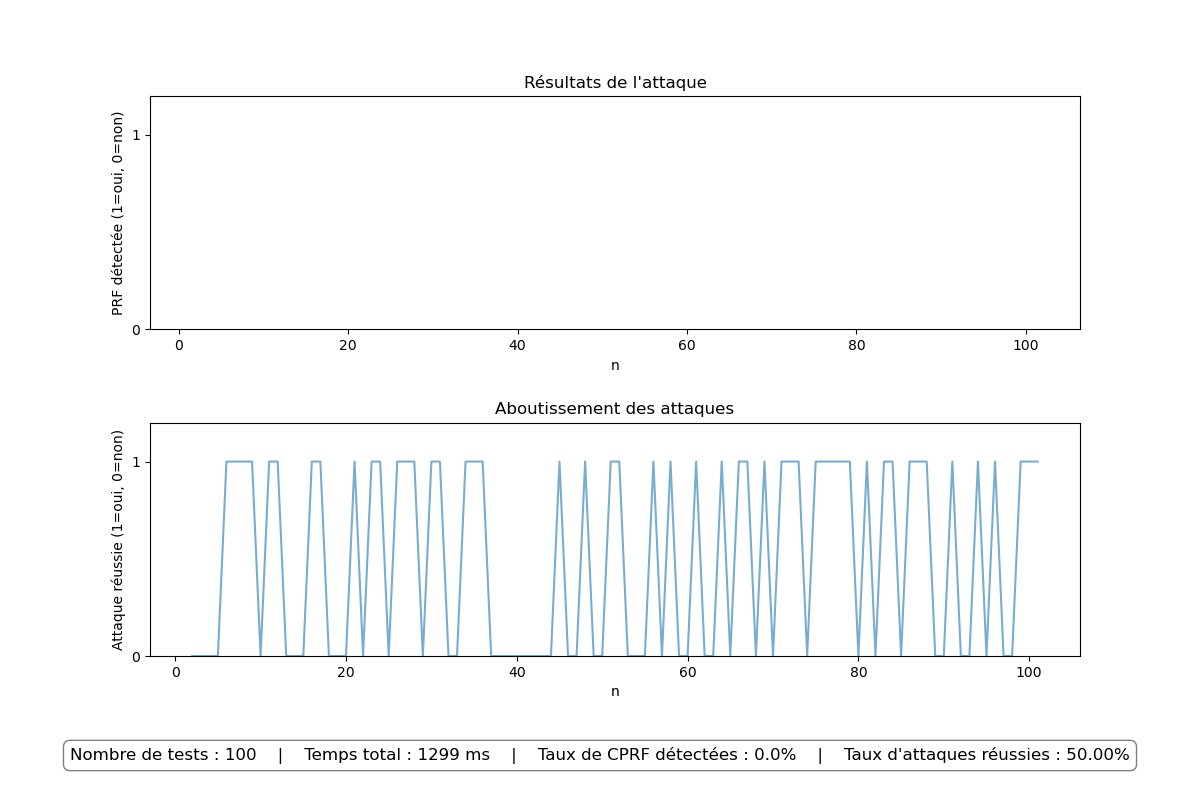
\includegraphics[width=0.7\textwidth]{./images/stat2.png}
\caption{Attaque version hachée avec SHA-256}
\label{fig:stat2}
\end{figure}

\begin{figure}[H]
\centering
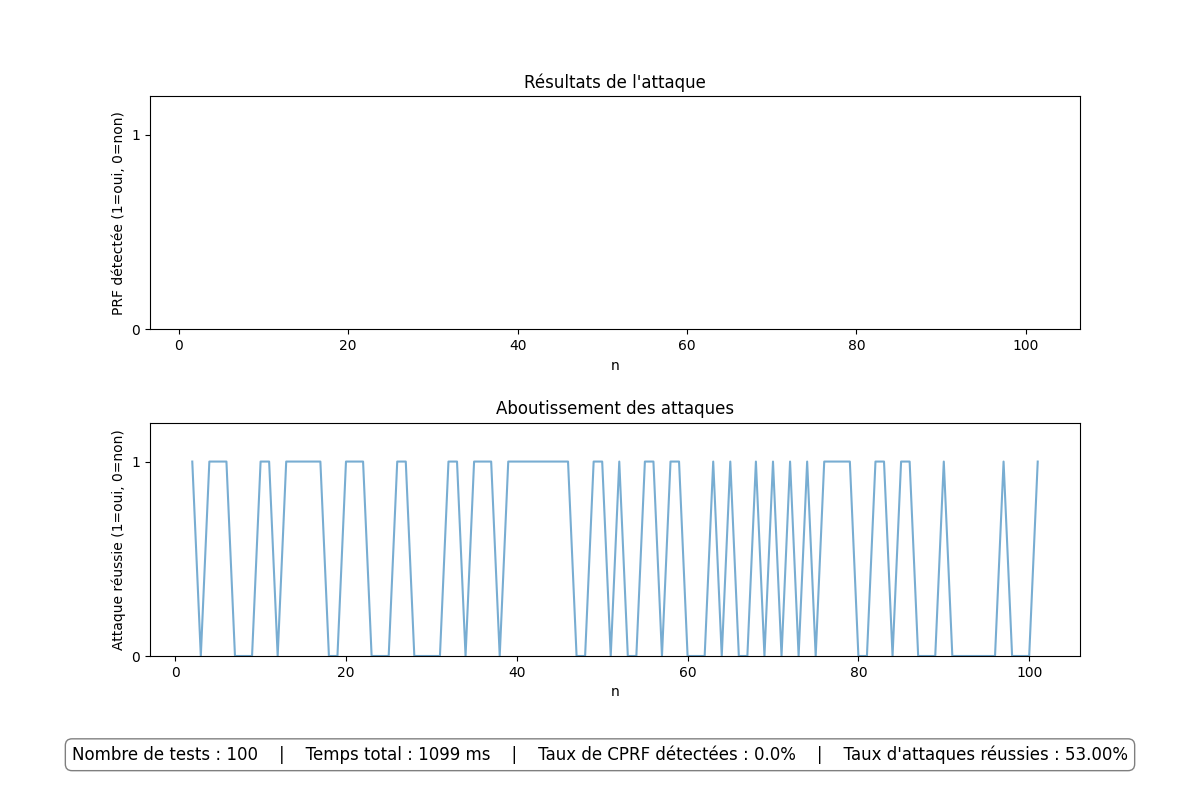
\includegraphics[width=0.7\textwidth]{./images/stat3.png}
\caption{Attaque version hachée avec lazy sampling}
\label{fig:stat3}
\end{figure}

\begin{figure}[H]
\centering
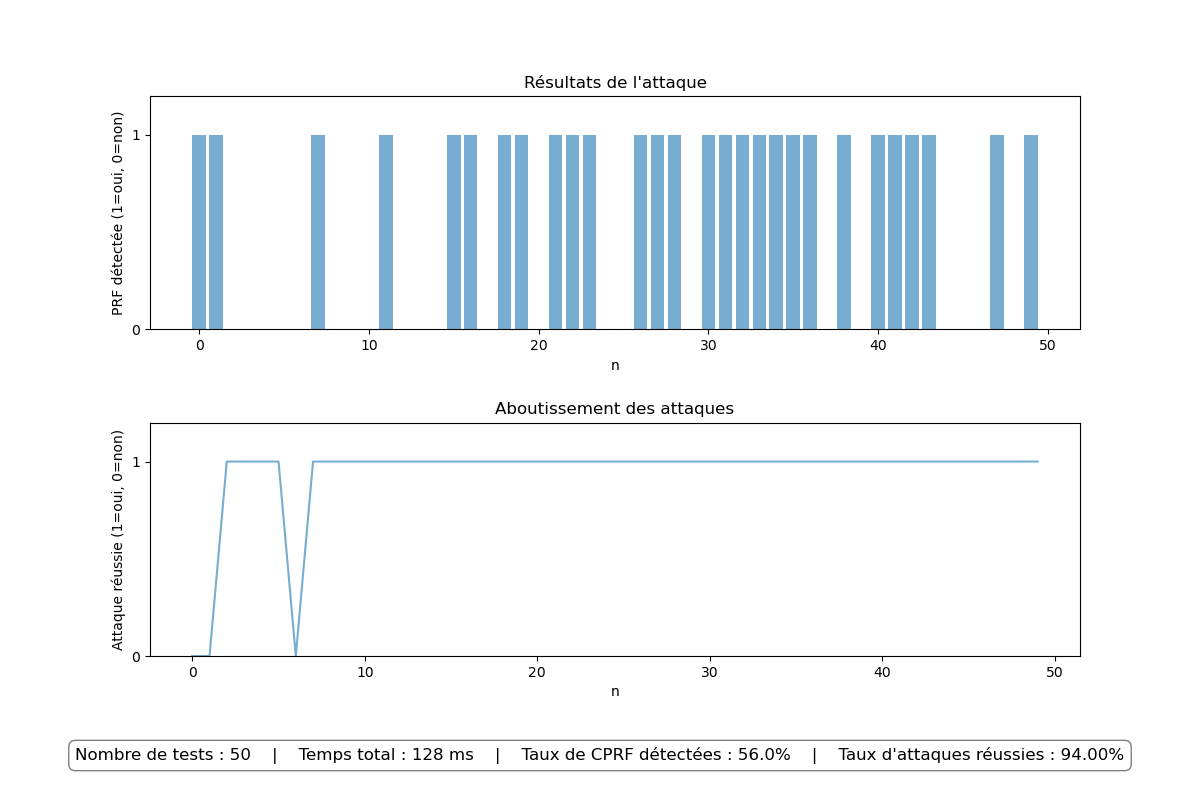
\includegraphics[width=0.7\textwidth]{./images/stat4.png}
\caption{Attaque Fweak}
\label{fig:stat4}
\end{figure}

\section{Guide d'utilisation}

\subsubsection*{Compiler}

\begin{verbatim}
make
\end{verbatim}

\subsubsection*{Exécuter}

\begin{verbatim}
./start.sh <mode> [parameters]
\end{verbatim}

\begin{center}
\begin{tabular}{|l|l|l|}
\hline
\textbf{Mode} & \textbf{Paramètres} & \textbf{Description} \\
\hline
\texttt{-n} & \texttt{<size>} & CPRF normale, nombre de tests \\
\hline
\texttt{-h} & \texttt{<size>} & CPRF hachée (SHA-256), nombre de tests \\
\hline
\texttt{-l} & \texttt{<size>} & Lazy sampling, nombre de tests \\
\hline
\texttt{-f} & \texttt{<tries> <N> <M>} & Mode FWEAK : nombre de tentatives, taille N et M \\
\hline
\end{tabular}
\end{center}

\subsubsection*{Afficher les courbes}

\begin{verbatim}
python3 display.py
\end{verbatim}

\appendix

\begin{thebibliography}{9}

\bibitem{BMO17}
E. Bost, B. Minaud, and O. Ohrimenko,
\textit{Forward and Backward Private Searchable Encryption from
Constrained Cryptographic Primitives},
ACM CCS 2017.

\bibitem{CJ25}
K. Cheng and J. Jaeger,
\textit{Adaptive Security for Constrained PRFs},
2025.

\end{thebibliography}

\end{document}
